% id: 103-18
% book: 100발100중 3-2 기말 · 01 3-2 기말(원의 성질·통계·부록)
% section: 족집게 마무리 객관식 80선
% figure: crop:fig-103-18.png
% answer: ③
% answer_source: 답지(빠른정답)
% variant_level: 0 (원본 전사)
% 이 파일은 build.mjs 가 items.json 에서 만든다. 고칠 때는 items.json 을 고친다.
\smash{\raisebox{1.5mm}{\dmkichul{100발100중 3-2 기말 103쪽 18번}}}
\noindent\begin{minipage}[t]{0.58\linewidth}\vspace{0pt}\raggedright 그림에서 네 점~$\pt{A}$, $\pt{B}$, $\pt{C}$, $\pt{D}$가 한 원 위에 있도록 하는 $\angle x$, $\angle y$의 크기를 각각 구하면?\end{minipage}\hfill\begin{minipage}[t]{0.4\linewidth}\vspace{0pt}\centering 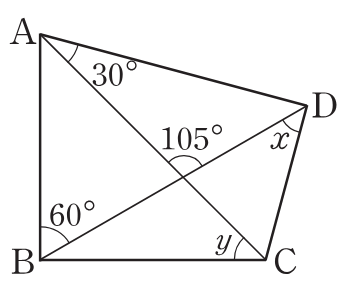
\includegraphics[width=82.9pt]{figures/fig-103-18.png}\end{minipage}\par
\begin{choicesv}{$\angle x=35^\circ$, $\angle y=45^\circ$}{$\angle x=35^\circ$, $\angle y=55^\circ$}{$\angle x=45^\circ$, $\angle y=45^\circ$}{$\angle x=45^\circ$, $\angle y=55^\circ$}{$\angle x=55^\circ$, $\angle y=35^\circ$}\end{choicesv}
